\chapter{Conception du syst\`eme}
\label{chap:conception-systeme}

Ce chapitre pr\'esente la conception fonctionnelle et dynamique du syst\`eme.
Les diagrammes utilisent une notation anglaise coh\'erente avec les noms des
composants et des interfaces du projet. Ils sont ins\'er\'es sous forme
vectorielle afin que le texte reste net à l'impression et au zoom.

\section{Vue fonctionnelle}

Le diagramme de cas d'utilisation de la figure~\ref{fig:use-cases} d\'elimite le
syst\`eme observ\'e. Il distingue l'op\'erateur humain du producteur externe de
flux ou d'\'ev\'enements IoT. L'attaquant n'est pas mod\'elis\'e comme acteur du
syst\`eme: les actions d'analyse portent sur les observations et alertes d\'ej\`a
collect\'ees.

\clearpage
\begin{landscape}
  \centering
  \vspace*{\fill}
  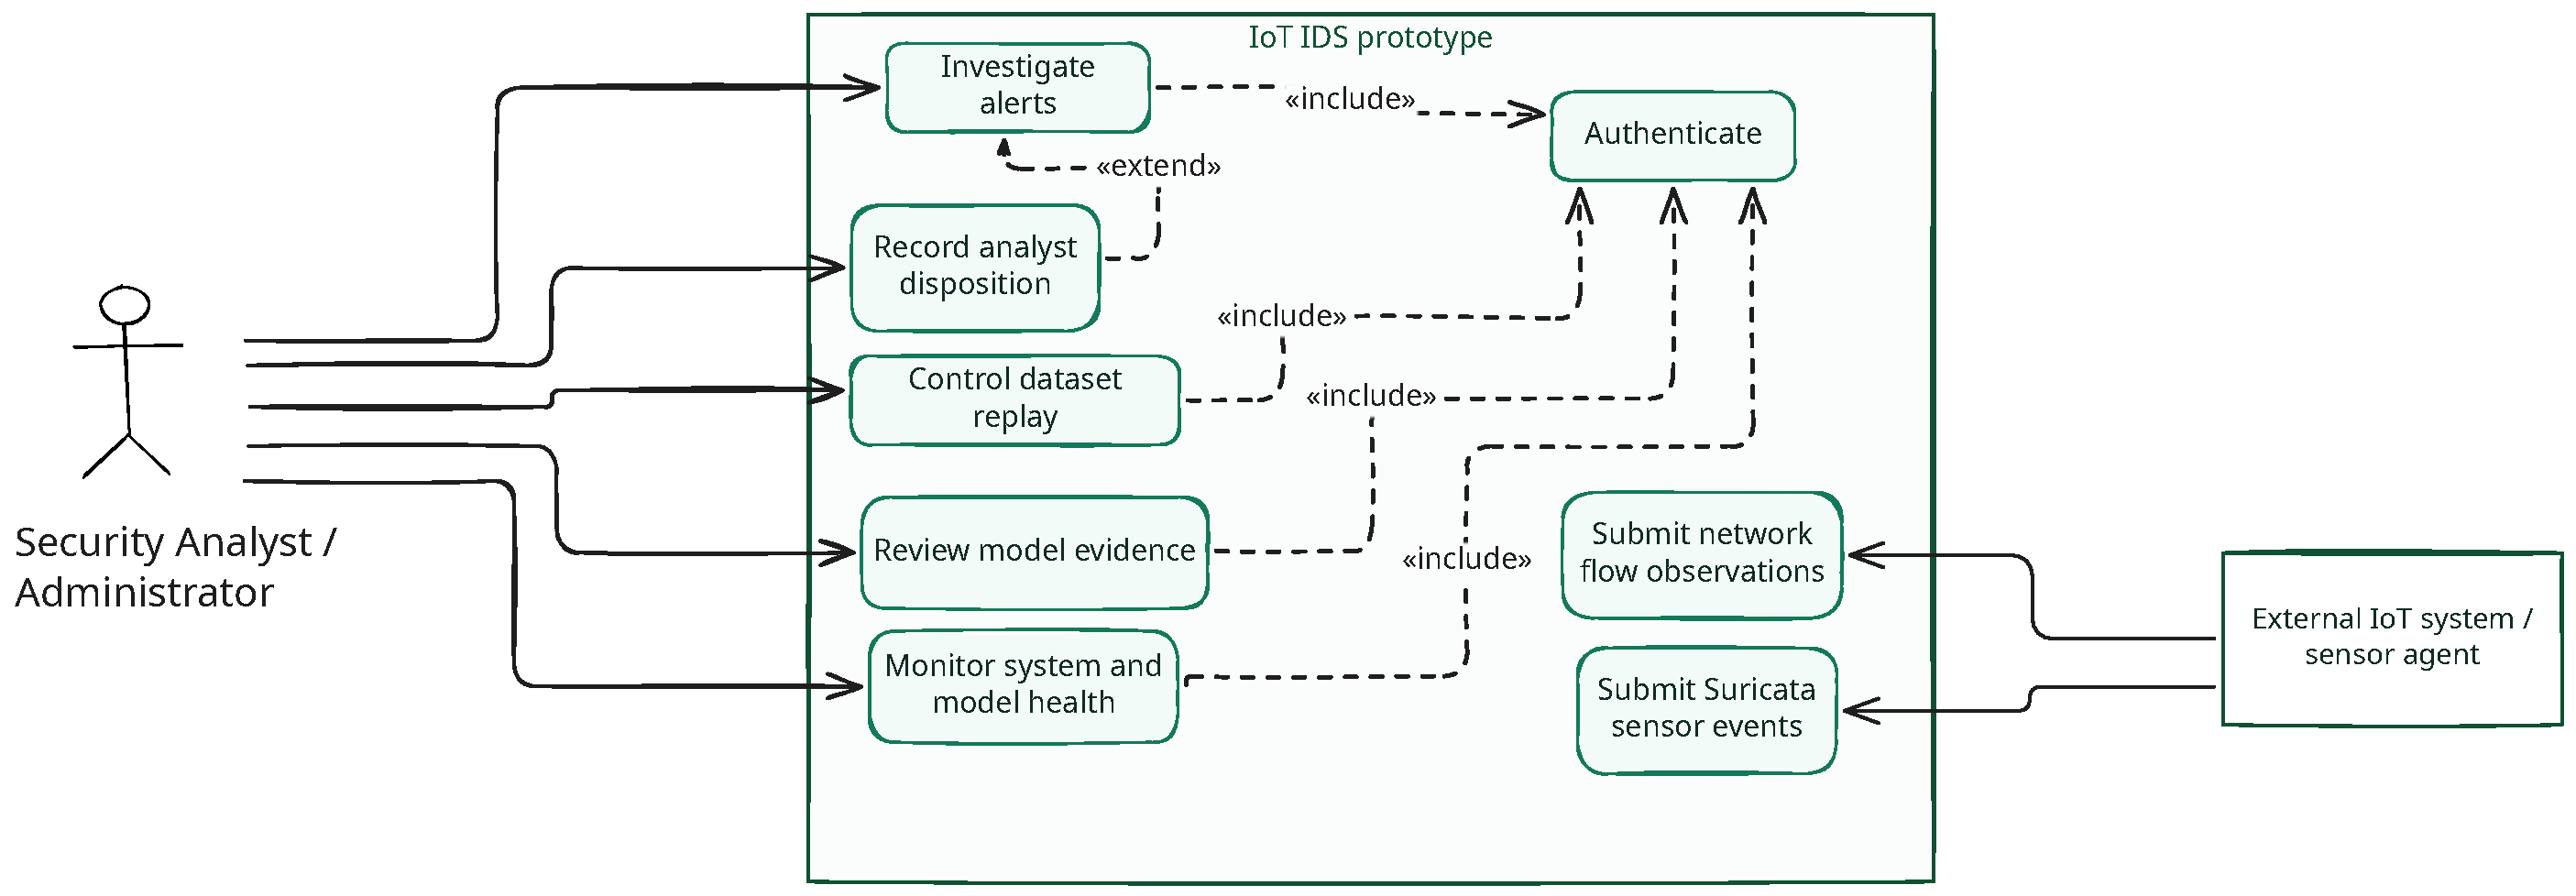
\includegraphics[width=0.98\linewidth,height=0.74\textheight,keepaspectratio]{../diagrams/rendered/01-use-cases-user.pdf}
  \captionsetup{hypcap=false}
  \captionof{figure}{Cas d'utilisation du syst\`eme de d\'etection}
  \label{fig:use-cases}
  \vspace*{\fill}
\end{landscape}

\clearpage
\section{Mod\`ele du domaine}

La vue principale de la figure~\ref{fig:domain-classes} organise les concepts
m\'etier persistants: observations de flux, pr\'edictions, alertes, jeux de
donn\'ees et mod\`eles. Les associations expriment les relations structurelles;
les d\'etails propres aux traitements asynchrones sont isol\'es dans des vues
compl\'ementaires pour conserver une lecture exploitable sur une page A4.

\begin{figure}[htbp]
  \centering
  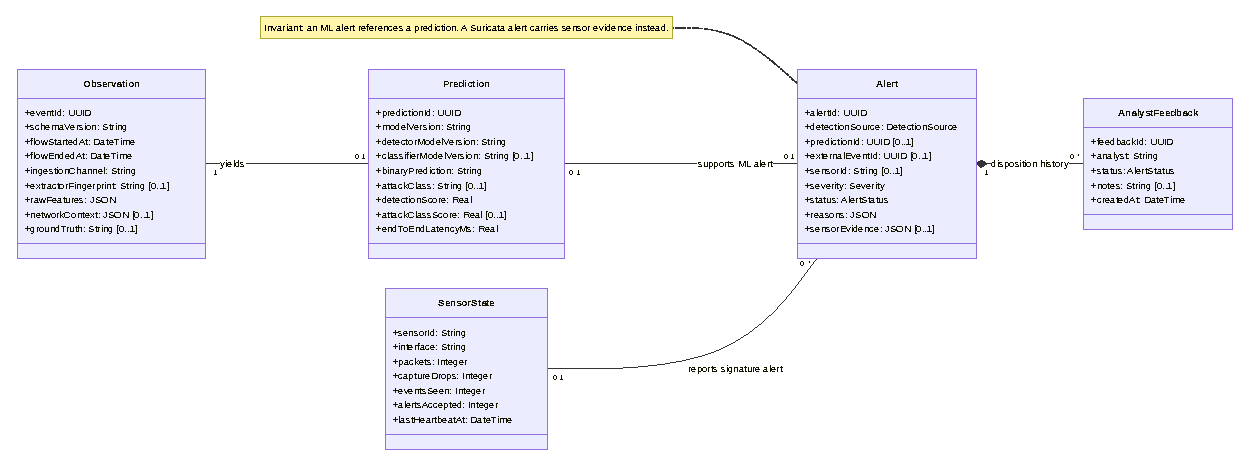
\includegraphics[width=\textwidth,height=0.68\textheight,keepaspectratio]{../diagrams/rendered/03-domain-classes.pdf}
  \caption{Diagramme de classes du domaine principal}
  \label{fig:domain-classes}
\end{figure}

\begin{figure}[htbp]
  \centering
  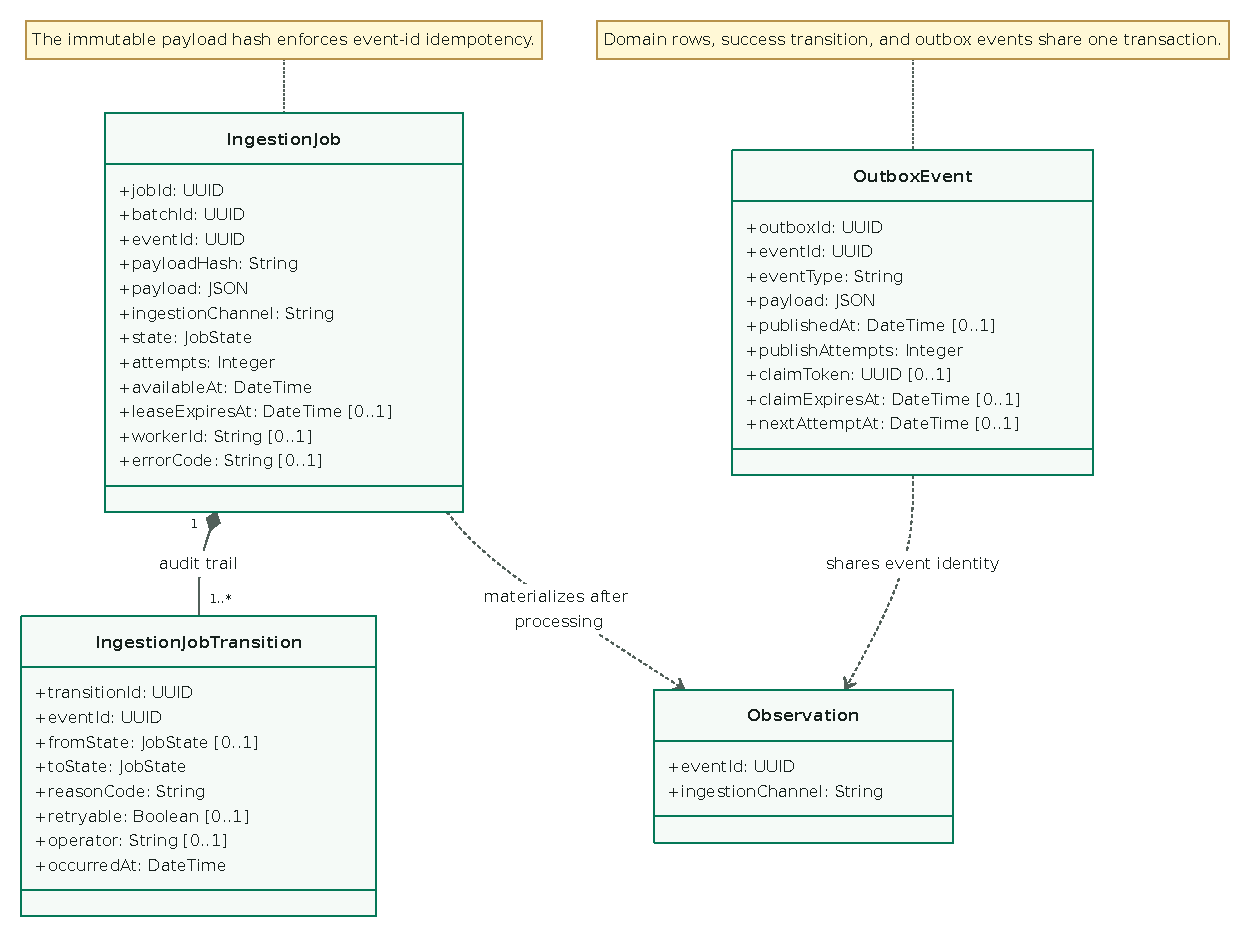
\includegraphics[width=\textwidth,height=0.68\textheight,keepaspectratio]{../diagrams/rendered/03b-ingestion-classes.pdf}
  \caption{Classes associ\'ees à l'ingestion durable}
  \label{fig:ingestion-classes}
\end{figure}

\begin{figure}[htbp]
  \centering
  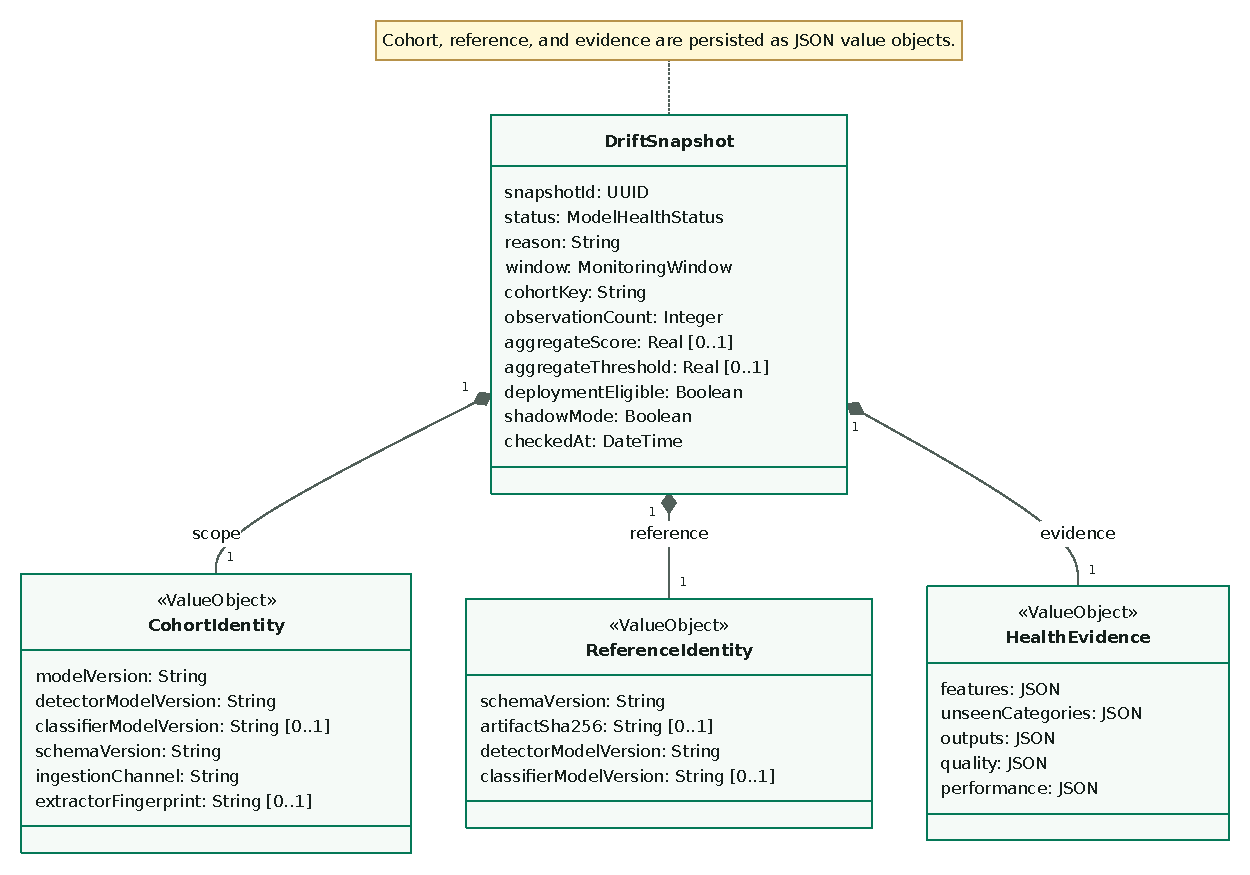
\includegraphics[width=\textwidth,height=0.68\textheight,keepaspectratio]{../diagrams/rendered/03c-model-health-classes.pdf}
  \caption{Classes associ\'ees au suivi de l'\'etat des mod\`eles}
  \label{fig:model-health-classes}
\end{figure}

\clearpage
\section{Ingestion durable des observations}

La figure~\ref{fig:ingestion-sequence} s\'epare l'acceptation HTTP, le traitement
asynchrone et la diffusion temps r\'eel. Les transactions rendent visibles les
fronti\`eres d'atomicit\'e, tandis que les fragments alternatifs explicitent le
rejet, la r\'eussite et la reprise apr\`es erreur. Le cycle de vie persistant
correspondant est synth\'etis\'e par la figure~\ref{fig:ingestion-states}.

\begin{figure}[htbp]
  \centering
  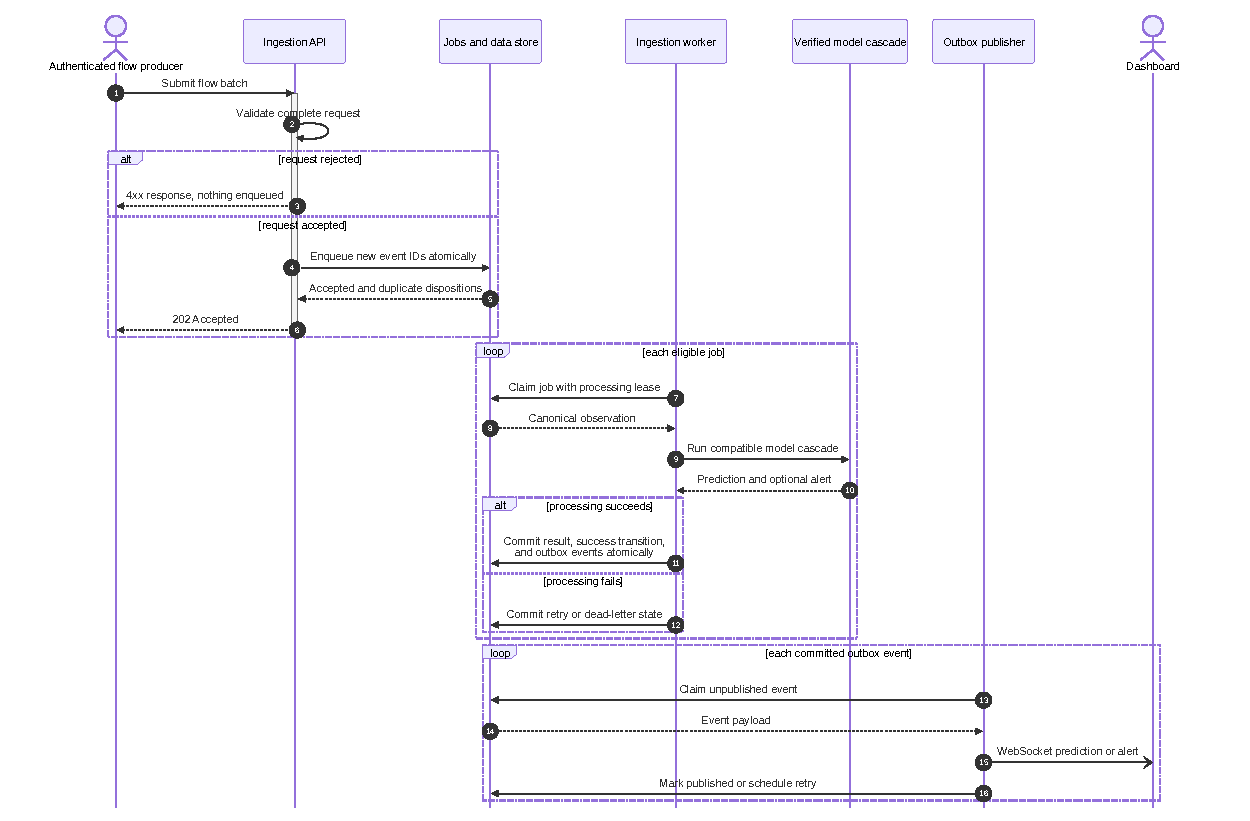
\includegraphics[width=\textwidth,height=0.68\textheight,keepaspectratio]{../diagrams/rendered/02-ingestion-sequence.pdf}
  \caption{S\'equence d'ingestion durable et de diffusion des r\'esultats}
  \label{fig:ingestion-sequence}
\end{figure}

\begin{figure}[htbp]
  \centering
  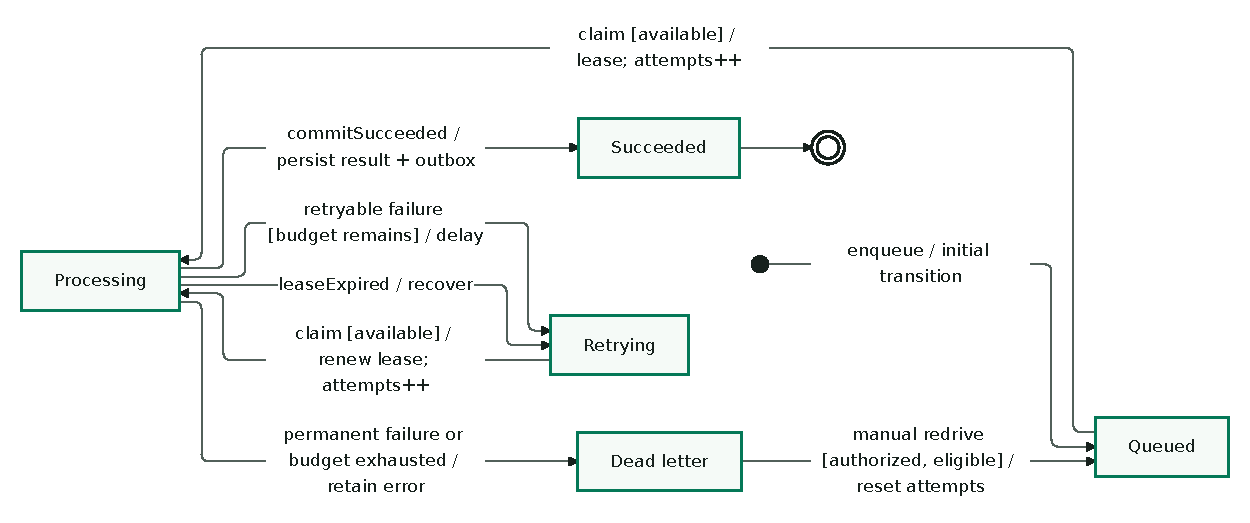
\includegraphics[width=\textwidth,height=0.68\textheight,keepaspectratio]{../diagrams/rendered/04-ingestion-states.pdf}
  \caption{Machine à \'etats d'un travail d'ingestion}
  \label{fig:ingestion-states}
\end{figure}

\clearpage
\section{Authentification et contr\^ole d'acc\`es}

La figure~\ref{fig:authentication-sequence} d\'ecrit l'\'emission d'une session,
son utilisation sur une ressource prot\'eg\'ee et le refus des requ\^etes qui ne
satisfont pas les contr\^oles d'identit\'e ou d'autorisation.

\begin{figure}[htbp]
  \centering
  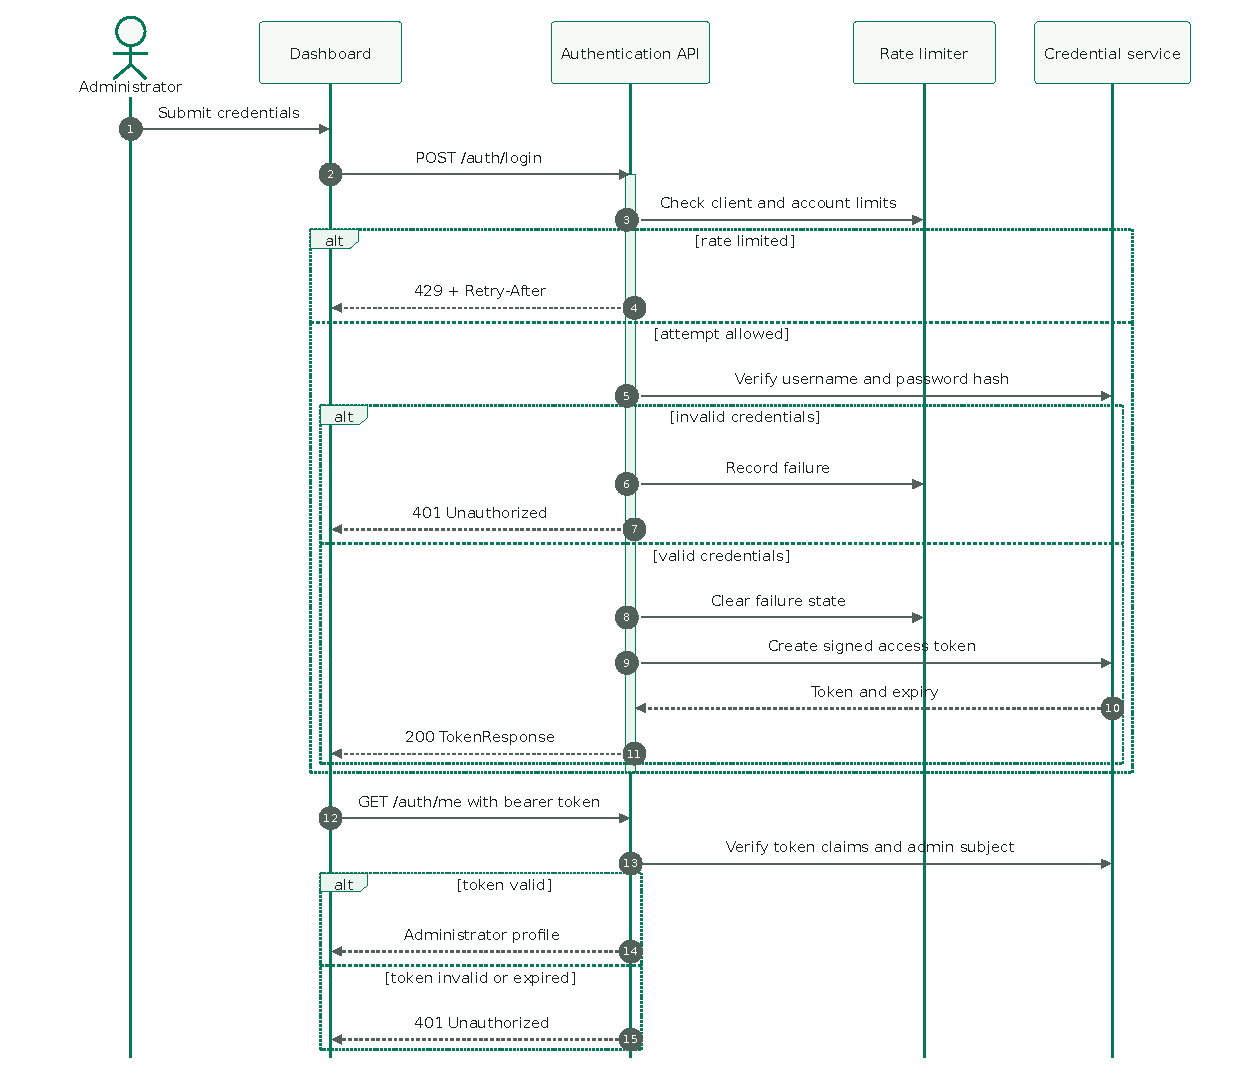
\includegraphics[width=\textwidth,height=0.68\textheight,keepaspectratio]{../diagrams/rendered/06-authentication-sequence.pdf}
  \caption{S\'equence d'authentification et d'autorisation}
  \label{fig:authentication-sequence}
\end{figure}

\clearpage
\section{Pr\'ediction et rejeu de donn\'ees}

Deux parcours sont distingu\'es. La pr\'ediction synchrone de la
figure~\ref{fig:synchronous-prediction} fournit une r\'eponse imm\'ediate pour une
observation. Le rejeu de la figure~\ref{fig:dataset-replay} traite une suite
d'observations sous le contr\^ole de l'utilisateur, avec progression et
possibilit\'e d'arr\^et.

\begin{figure}[htbp]
  \centering
  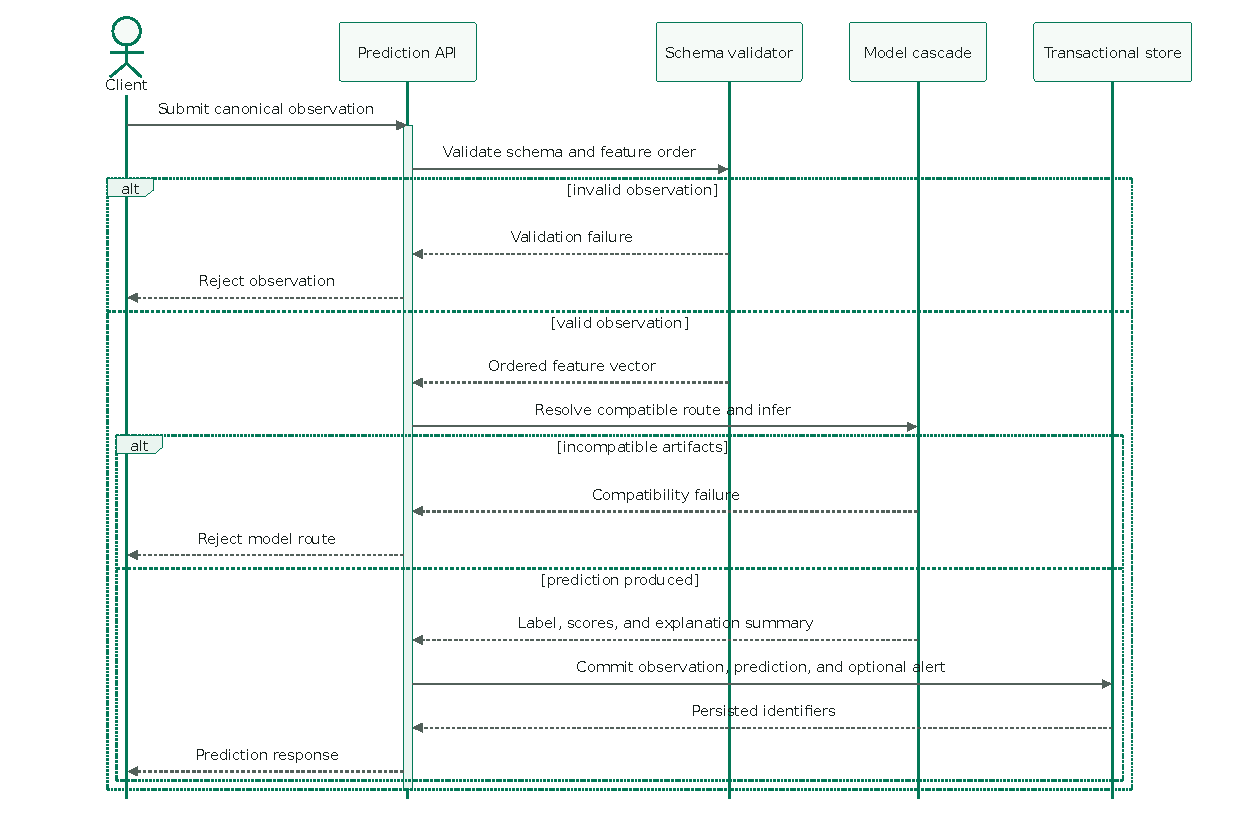
\includegraphics[width=\textwidth,height=0.68\textheight,keepaspectratio]{../diagrams/rendered/07-synchronous-prediction-sequence.pdf}
  \caption{S\'equence de pr\'ediction synchrone}
  \label{fig:synchronous-prediction}
\end{figure}

\begin{figure}[htbp]
  \centering
  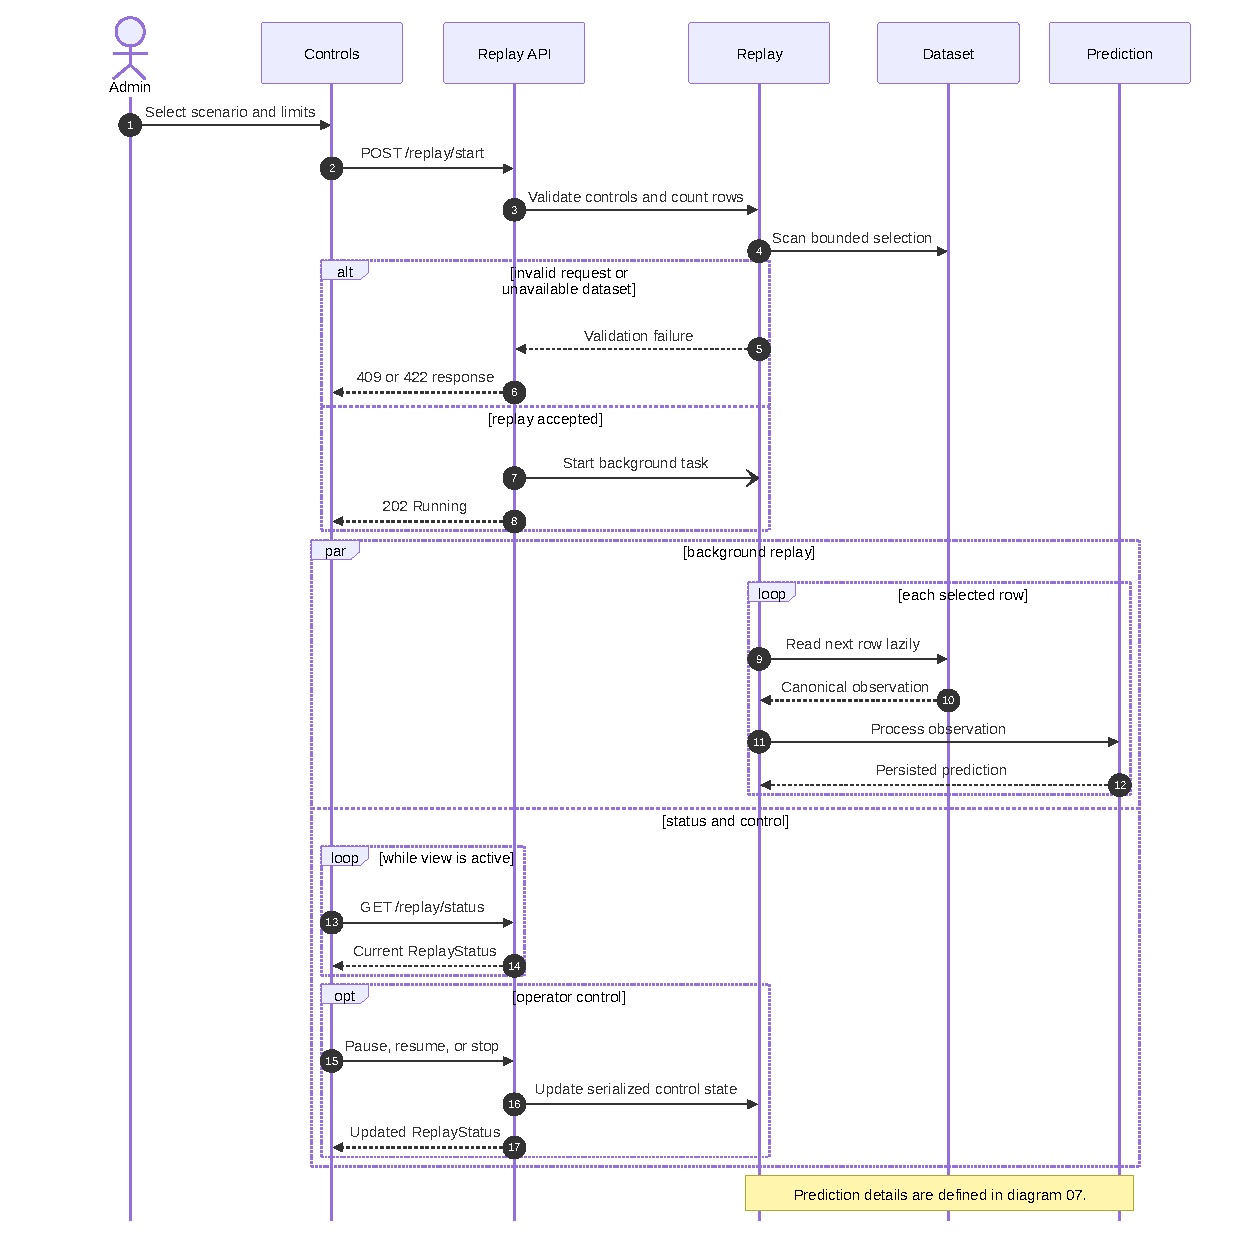
\includegraphics[width=\textwidth,height=0.68\textheight,keepaspectratio]{../diagrams/rendered/08-dataset-replay-sequence.pdf}
  \caption{S\'equence de rejeu contr\^ol\'e d'un jeu de donn\'ees}
  \label{fig:dataset-replay}
\end{figure}

\clearpage
\section{Investigation des alertes}

L'investigation d'une alerte est d\'etaill\'ee dans la
figure~\ref{fig:alert-investigation}. Elle relie la consultation des preuves à
la d\'ecision de l'analyste et conserve une trace de l'interpr\'etation humaine
du r\'esultat automatique.

\begin{figure}[htbp]
  \centering
  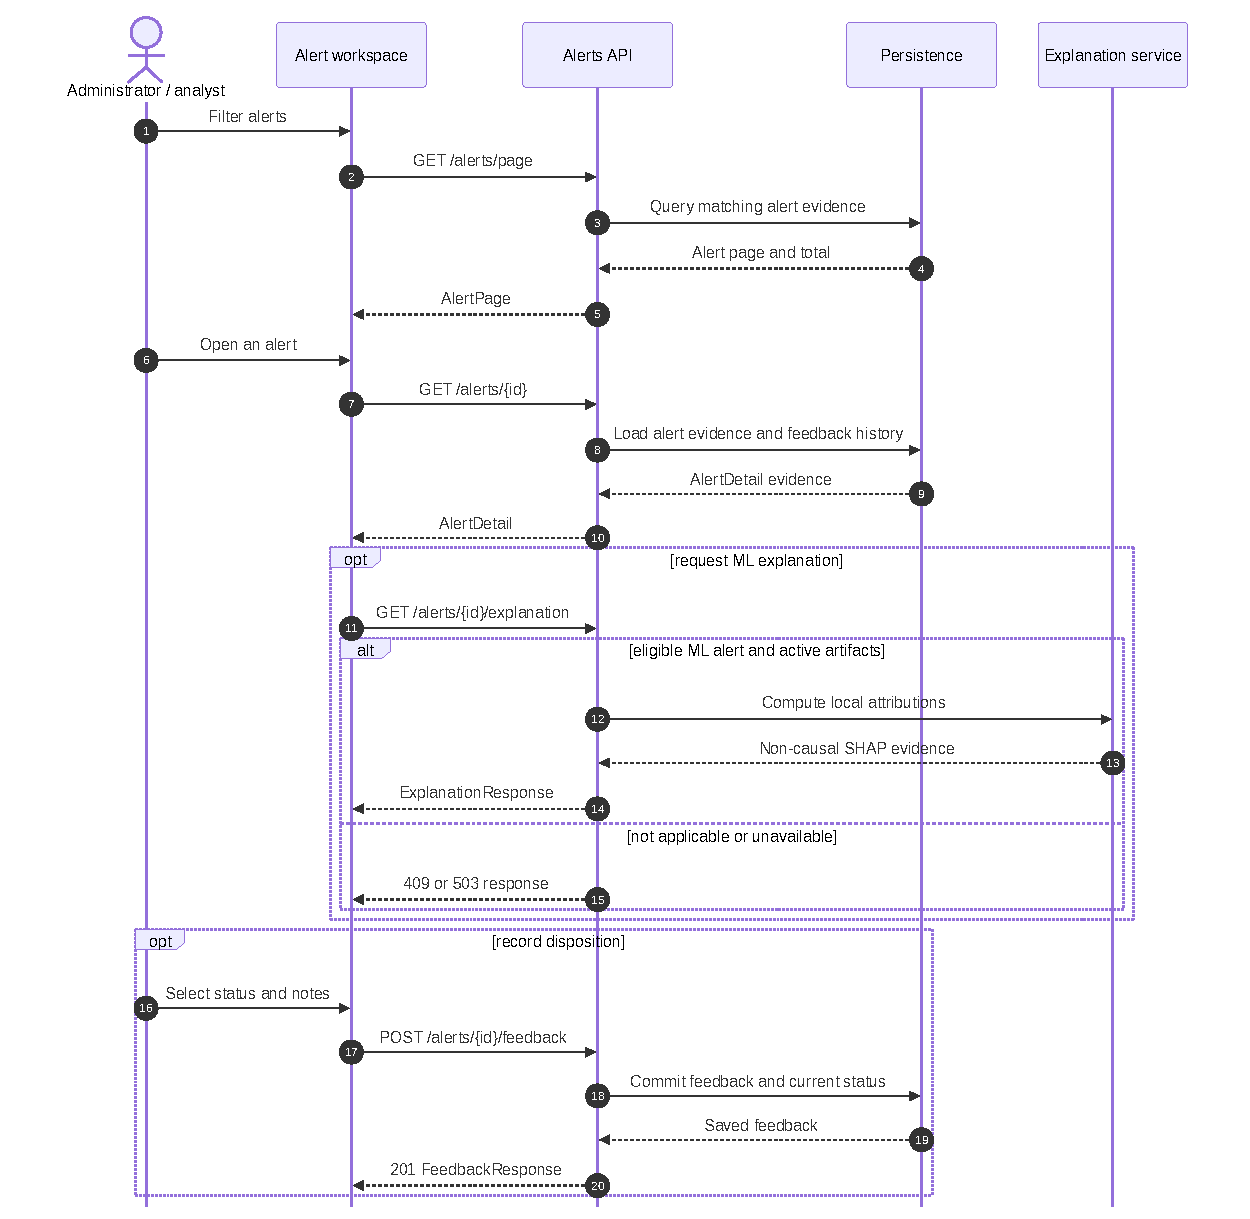
\includegraphics[width=\textwidth,height=0.68\textheight,keepaspectratio]{../diagrams/rendered/09-alert-investigation-sequence.pdf}
  \caption{S\'equence d'investigation et de qualification d'une alerte}
  \label{fig:alert-investigation}
\end{figure}

\clearpage
\section{Int\'egration du capteur Suricata}

La figure~\ref{fig:suricata-sequence} repr\'esente le capteur comme un syst\`eme
externe. L'adaptateur transforme ses \'ev\'enements en observations compatibles
avec le contrat d'ingestion, puis applique la politique de reprise pr\'evue en
cas d'indisponibilit\'e.

\begin{figure}[htbp]
  \centering
  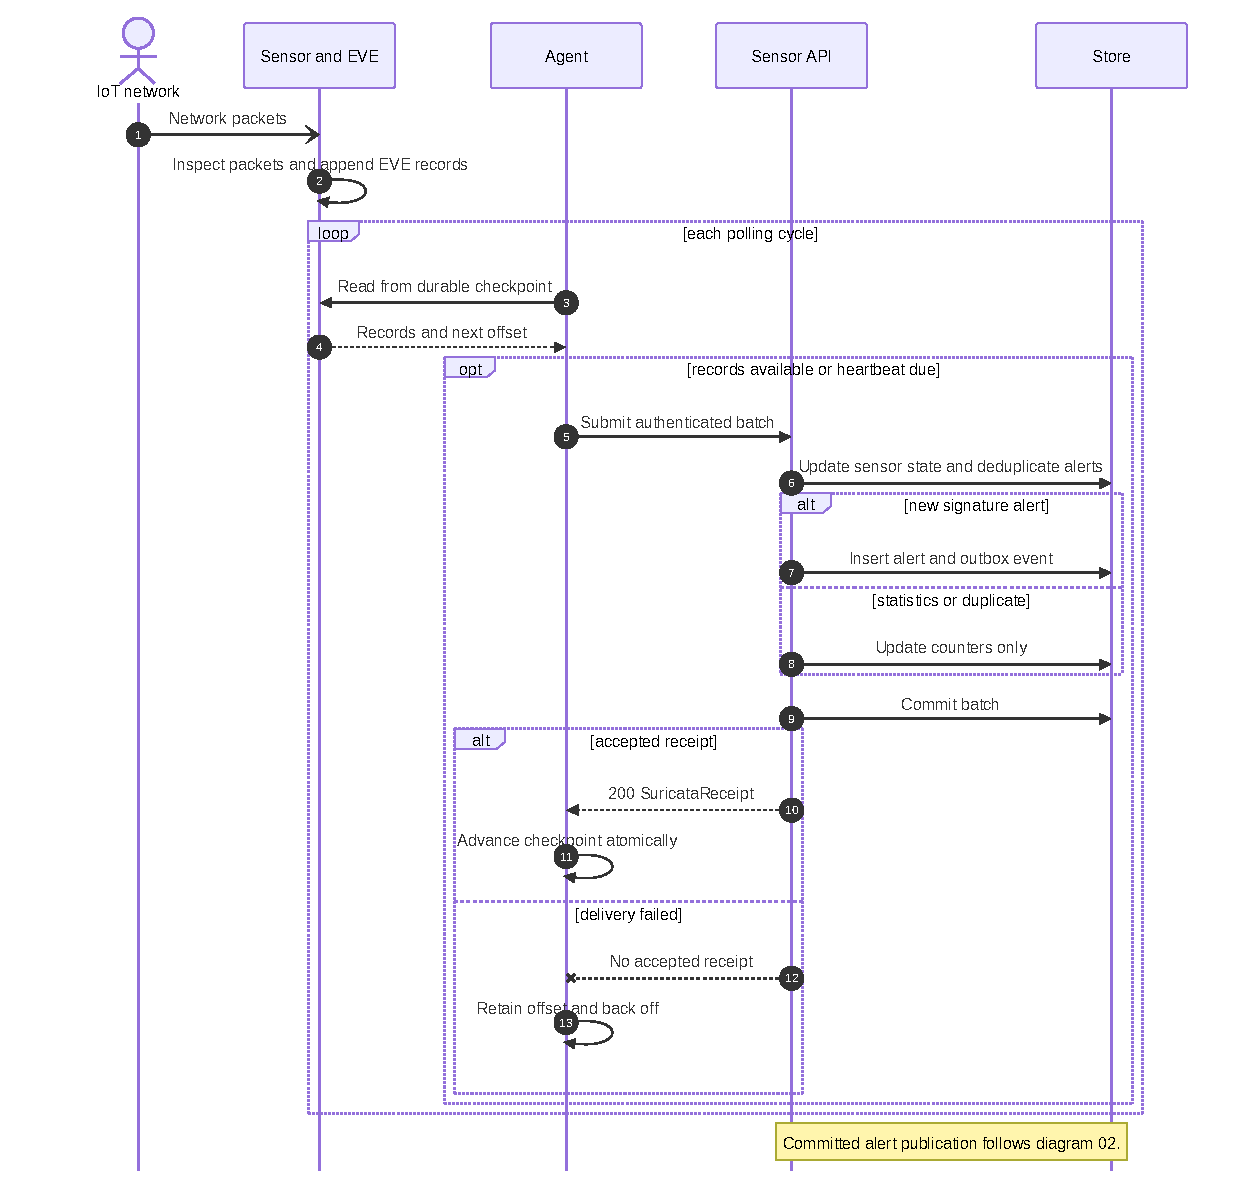
\includegraphics[width=\textwidth,height=0.68\textheight,keepaspectratio]{../diagrams/rendered/10-suricata-sensor-sequence.pdf}
  \caption{S\'equence d'int\'egration des \'ev\'enements Suricata}
  \label{fig:suricata-sequence}
\end{figure}

\clearpage
\section{Surveillance de la sant\'e des mod\`eles}

Le parcours de la figure~\ref{fig:model-health-sequence} rassemble les mesures
n\'ecessaires à l'examen d'un mod\`ele en service et à la restitution de son
\'etat dans l'interface d'administration.

\begin{figure}[htbp]
  \centering
  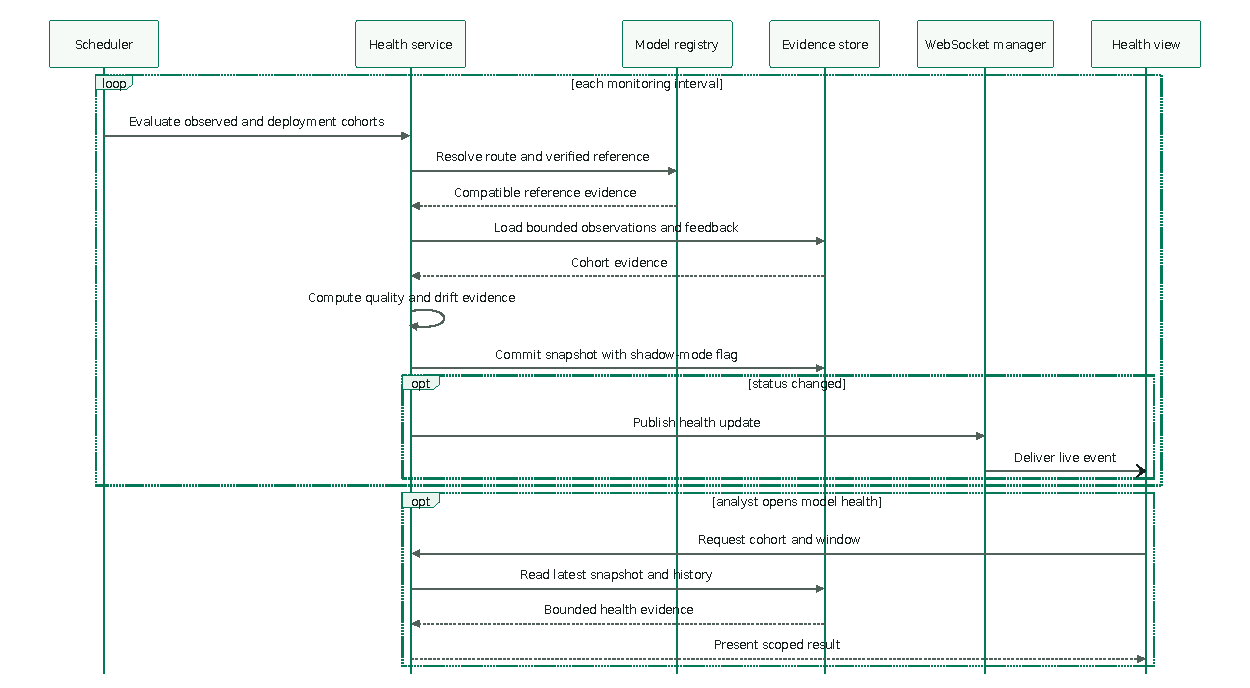
\includegraphics[width=\textwidth,height=0.68\textheight,keepaspectratio]{../diagrams/rendered/11-model-health-sequence.pdf}
  \caption{S\'equence de consultation de la sant\'e d'un mod\`ele}
  \label{fig:model-health-sequence}
\end{figure}

\section{Conclusion}

La d\'ecomposition en vues fonctionnelle, structurelle et dynamique limite la
densit\'e de chaque diagramme tout en couvrant les fonctions majeures du syst\`eme.
Les fronti\`eres externes, les responsabilit\'es des composants et les sc\'enarios
d'erreur sont ainsi visibles sans reproduire les d\'etails d'impl\'ementation dans
une seule figure surcharg\'ee.
